%###
\begin{frame}{Introduction}{What is a sparse grid?}

    A \textbf{numerical discretization technique} that can be used in a wide range of computaitonal problems:
    \begin{itemize}[<+->]
        \item Interpolation
        \item Regression
        \item Classification
        \item Density estimation
        \item Quadrature
        \item Uncertainty Quantification
        \item Solution of Partial Differential Equations
        \item \ldots
    \end{itemize}

\end{frame}
%###

%###
\begin{frame}{Introduction}{Why do we need sparse grids?}
    In general solution on a \emph{full grid} (i.e. a grid with all points) is only feasible if the dimensionality of the problem is low ($d=1,2,3$)

    \pause

    However, in some cases, the dimensionality of the problem is high ($d\ge 4$) and the solution on a \emph{full grid} is not feasible.

    \pause

    This dilemma is called \emph{curse of dimensionality} and is the reason why sparse grids are used in many scientific applications.

\end{frame}
%###

\begin{frame}{Introduction}{A brief comparision}
    \begin{columns}
        \begin{column}[]{0.6\textwidth}
            The required grid points and the Euclidian norm of the interpolation error on a regular sparse grid and on a full grid is shown in the following table below for \(d\) dimensional space and grid level of \(n\).
            \vfill

            \resizebox{\textwidth}{!}{
                \begin{tabular}{l c c}
                    \multicolumn{1}{c}{} & Number of grid points & \multicolumn{1}{c}{L2 Norm of Interpolation Error} \\
                    \toprule
                    Full Grid            & \(O(2^{nd})\)         & \(O(2^{-2n})\)                                     \\
                    \midrule
                    Sparse Grid          & \(O(2^{n} n^{d-1})\)  & \(O(2^{-2n} n^{d-1})\)                             \\
                    \bottomrule
                \end{tabular}
            }
        \end{column}
        \pause
        \begin{column}[]{0.4\textwidth}
            \centering
            \resizebox{!}{0.7\textheight}{
                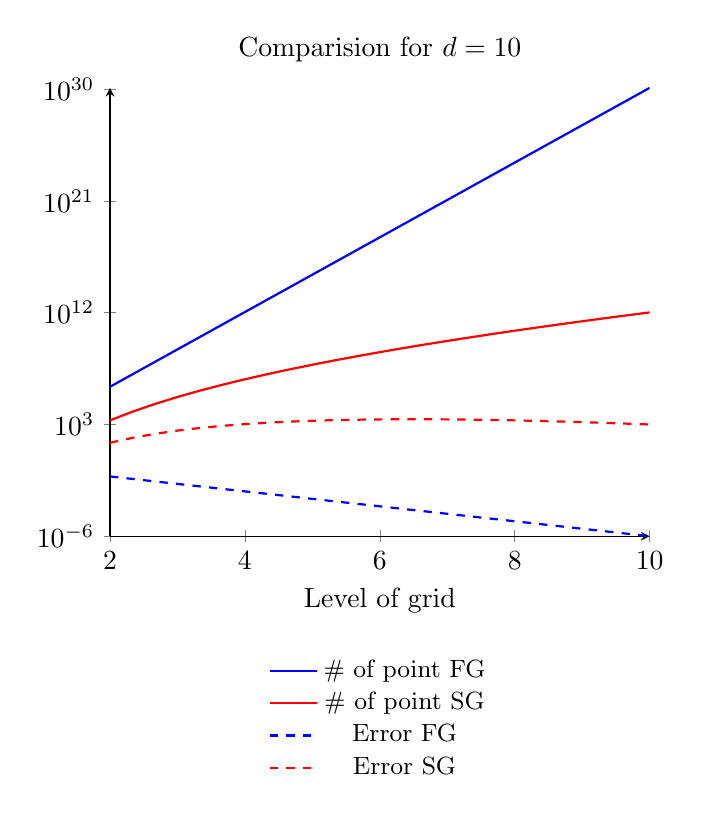
\begin{tikzpicture}
                    \begin{axis}[
                            axis x line=bottom,
                            axis y line=left,
                            xtick={2,4,...,16},
                            xlabel={Level of grid},
                            ymode = log,
                            domain=2:10,
                            legend style ={at={(0.5,-0.25)},anchor=north,font=\tiny,draw=none},
                            title={Comparision for $d=10$},
                        ]
                        \addplot [color=blue,thick] {2^(x*10)};
                        \addplot [color=red,thick] {2^x*x^9};
                        \addplot [color=blue,thick,dashed] {2^(-2*x)};
                        \addplot [color=red,thick,dashed] {2^(-2*x)*x^9};
                        \legend{\small{\# of point FG}, \small{\# of point SG}, \small{Error FG}, \small{Error SG}}
                    \end{axis}
                \end{tikzpicture}
            }
        \end{column}
    \end{columns}

\end{frame}

\begin{frame}{Introduction}{How they look?}

    \begin{columns}
        \begin{column}{0.5\textwidth}
            \begin{figure}
                \centering
                \includegraphics[width=\textwidth]{figures/full_grid_level_3.pdf}
            \end{figure}
        \end{column}
        \begin{column}{0.5\textwidth}
            \begin{figure}
                \centering
                \includegraphics[width=\textwidth]{figures/sparse_grid_level_3.pdf}
            \end{figure}
        \end{column}
    \end{columns}

\end{frame}

\begin{frame}{Introduction}{How they look?}

    \begin{columns}
        \begin{column}{0.5\textwidth}
            \begin{figure}
                \centering
                \includegraphics[width=\textwidth]{figures/full_grid_level_5.pdf}
            \end{figure}
        \end{column}
        \begin{column}{0.5\textwidth}
            \begin{figure}
                \centering
                \includegraphics[width=\textwidth]{figures/sparse_grid_level_5.pdf}
            \end{figure}
        \end{column}
    \end{columns}

\end{frame}